\begin{frame}{Nomad - Mise en contexte}
    \centering
    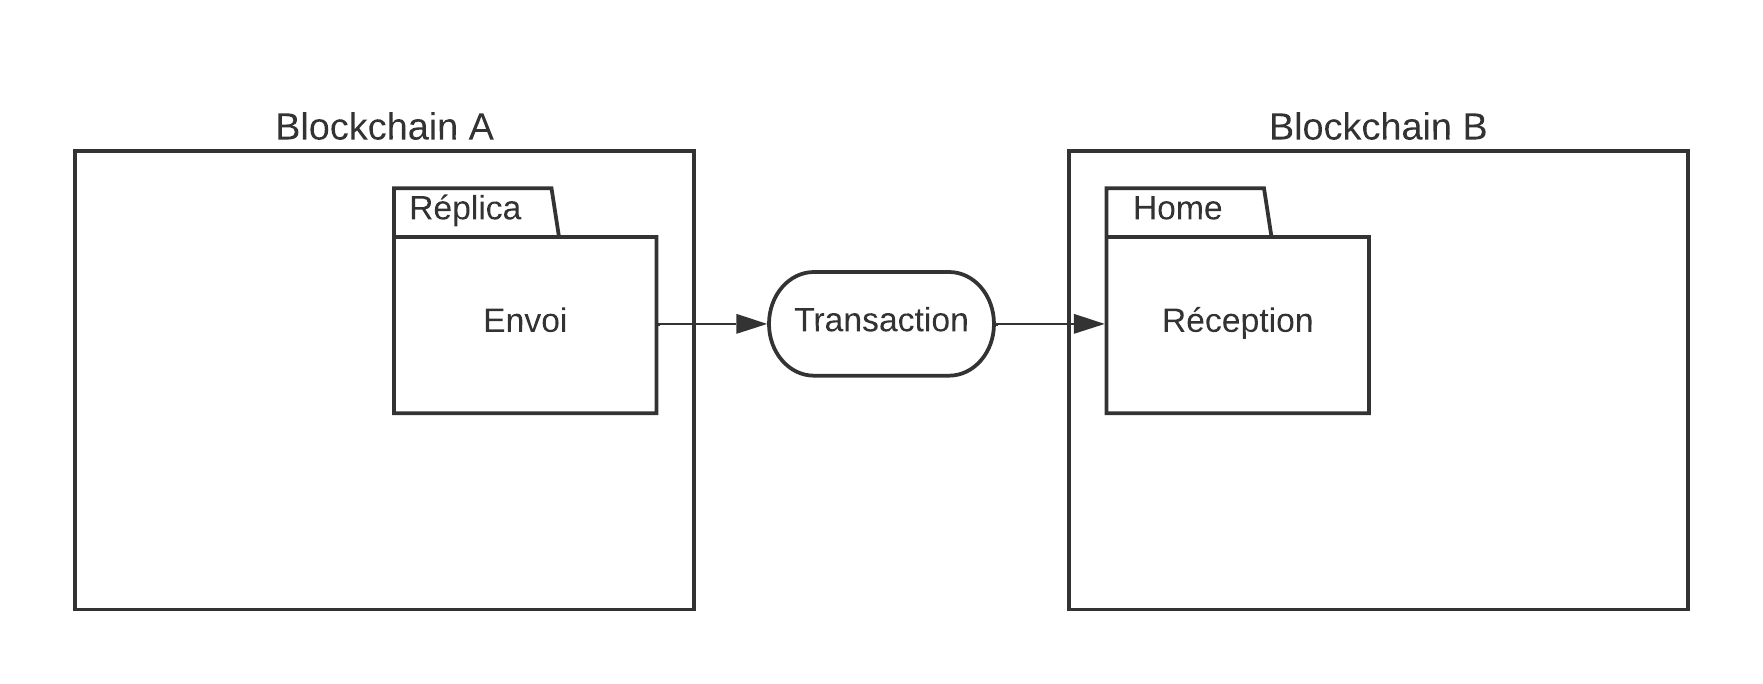
\includegraphics[scale = 0.8]{centralisation/img/nomad/nomad_contracts.png}
\end{frame}

%\begin{frame}{Le protocole Nomad}
%    \begin{block}{Mise en contexte}
%        \begin{itemize}
%            \item Protocole d'échange inter-blockchains.
%            \item Utilisation de \textit{smart contracts}.
%        \end{itemize}
%    \end{block}
%    \begin{block}{Les \textit{smart contracts}}
%        \begin{itemize}
%            \item \textit{Home} : "Boite d'envoi", déployé sur les blockchain source.
%            \item \textit{Replica} : "Boite de réception", déployé sur les blockchains de destination.
%        \end{itemize}
%    \end{block}
%\end{frame}

\begin{frame}{Nomad - Mise en contexte}
    \centering
    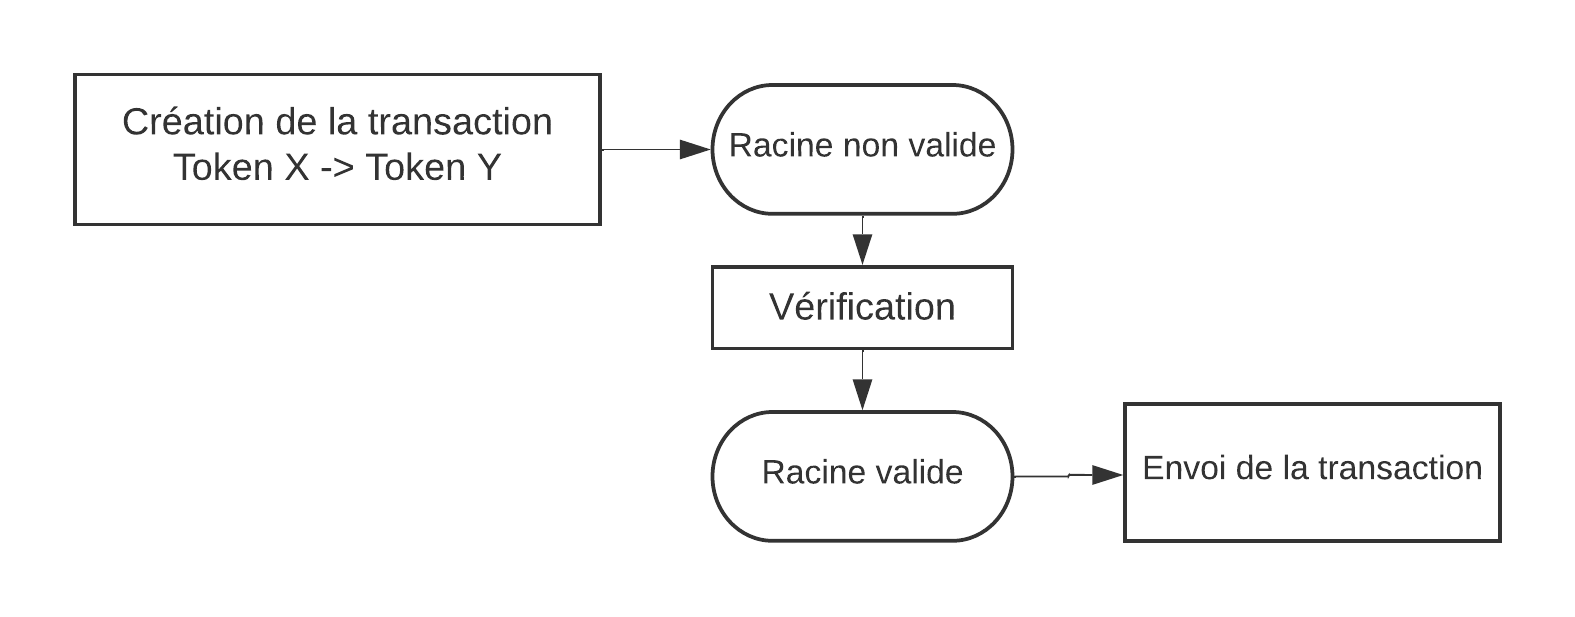
\includegraphics[scale = 0.9]{centralisation/img/nomad/nomad_fonc.png}
\end{frame}

%\begin{frame}{Le protocole Nomad}
%    \begin{block}{Fonctionnement d'une transaction}
%        \begin{itemize}
%            \item Création de la transaction.
%            \item Vérification du message par sa racine.
%            \item Accepte la racine.
%            \item Envoi.
%        \end{itemize}
%    \end{block}
%\end{frame}

\begin{frame}{Nomad - L'attaque}
    \begin{block}{Attaque sur les briges de Nomad}
        \begin{itemize}
            \item Premier Août 2022.
            \item Apparu après mise a jour utilisant la fonction \textit{process} pour vérifier la racine.
            \item 190 000 000 de dollars de liquidité volé.
        \end{itemize}
    \end{block}
    \begin{block}{L'erreur d'implémentation}
        \begin{itemize}
            \item Erreur d'implémentation sur \textit{Réplica}.
            \item Problème de vérification de racine.
            \item Possibilité de valider n'importe quel message.
        \end{itemize}
    \end{block}
\end{frame}

\begin{frame}{Nomad - L'attaque}
    \begin{block}{Erreur d'initialisation}
        \begin{itemize}
            \item Racine initialisée à $0$.
            \item Racine $0$ pré-approuvée.
        \end{itemize}
        $\rightarrow$ Tout message non vérifié sera valide.
    \end{block}
        \centering
        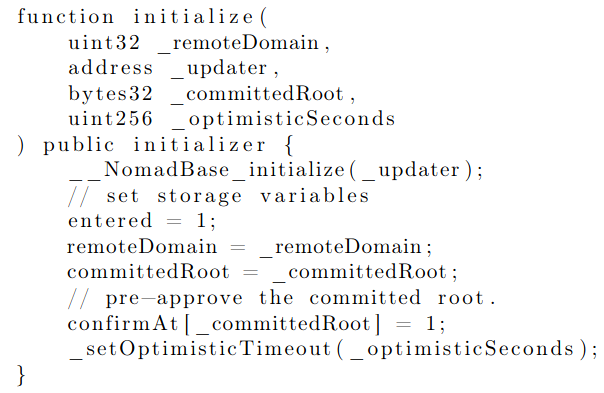
\includegraphics[scale = 0.35]{centralisation/img/nomad/nomad_code_hack.png}
\end{frame}

\begin{frame}{Nomad - L'attaque}
    \centering
    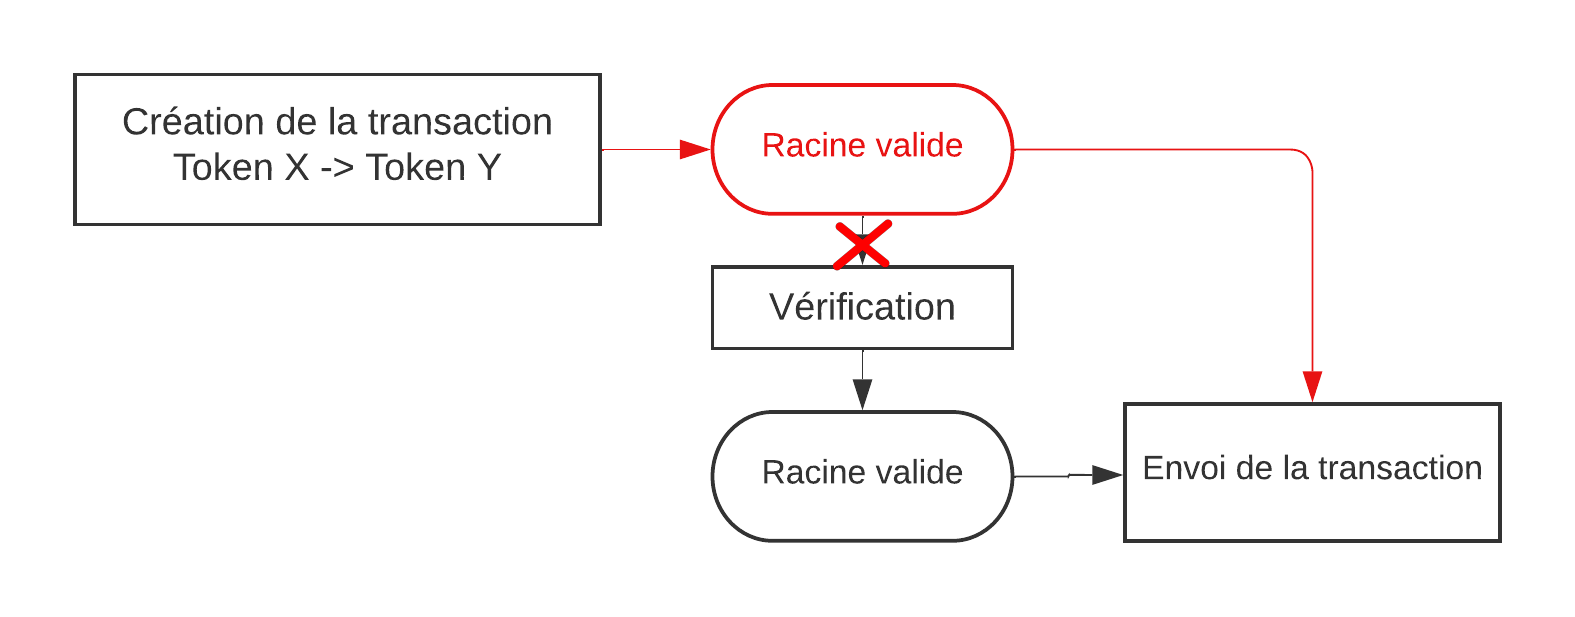
\includegraphics[scale = 0.9]{centralisation/img/nomad/nomad_hack.png}
\end{frame}

\begin{frame}{Nomad - Correctif}
    \begin{itemize}
        \item Correction le 3 septembre 2022
        \item La racine nulle n'est plus pré-approuvée.
    \end{itemize}
    \begin{figure}
        \centering
        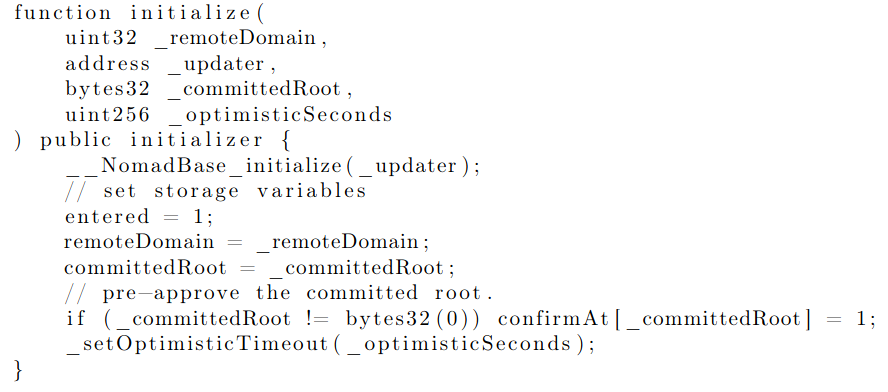
\includegraphics[scale = 0.35]{centralisation/img/nomad/nomad_code_fixed.png}
        \caption{Contrat Réplica corrigé}
    \end{figure}
\end{frame}